% Copyright (c) 2021 Eclipse Arrowhead Project
%
% This program and the accompanying materials are made available under the
% terms of the Eclipse Public License 2.0 which is available at
% http://www.eclipse.org/legal/epl-2.0.
%
% SPDX-License-Identifier: EPL-2.0

For a document, \GlossaryHyperRef{model}{model}, or other \GlossaryHyperRef{artifact}{artifact}, to be considered as conformant to this document, the following must be observed by that \textit{derived work}:

\begin{enumerate}
\item At least one of the concepts defined in this work must be part of that derived work.
\item The derived work must make it explicit what concepts are taken from this work.
	\begin{enumerate}
	\item How this is done most suitably depends on the type of derived work. A document may include a normative reference to this document, while a model may want to give all relevant \GlossaryHyperRef{entity}{entities} and \GlossaryHyperRef{relationship}{relationships} an \GlossaryHyperRef{attribute}{attribute} with the identity of this document, for example.
	\end{enumerate}
\item Every concept taken from this work must be represented by the name it is given here.
	\begin{enumerate}
	\item If important to be able to distinguish an Arrowhead concept from other such of relevance, concepts from this work may be qualified by the leading word ``Arrowhead'', as in, for example, ``Arrowhead system`` or ``Arrowhead service function''.
	\item Note that some concepts defined here are given more than one name. For example, \GlossaryHyperRef{function-program}{program function} and \GlossaryHyperRef{procedure-software}{software procedure} are declared to be synonyms in the glossary. When synonyms exist, only one of their entries in the glossary will have a definition. The name of that definition should be the name being used.
	\end{enumerate}
\item Concepts taken from this work may be \textit{specialized} or \textit{simplified}, but must never be \textit{contradicted}.
	\begin{enumerate}
	\item \textit{Specialization} means that more \GlossaryHyperRef{constraint}{constraints} are applied to it than are presented here. For example, a certain derived work may require that all devices have \GlossaryHyperRef{unit-compute}{compute units} supporting a certain instruction set, or that every \GlossaryHyperRef{system}{system} \GlossaryHyperRef{provider-service}{provides} a specific monitoring \GlossaryHyperRef{service}{service}, and so on.
	\item \textit{Simplification} means that entities, relationships or attributes introduced here are omitted due to being outside the scope of the derived work. For example, a technical document may not be concerned with \GlossaryHyperRef{role-stakeholder}{stakeholder roles}, while a model of certain types of local clouds may not be concerned with whether or not artifacts are \GlossaryHyperRef{resource}{resources} or not, and so on.
	\item \textit{Contradiction} means that a attribute or other constraint is introduced that makes it impossible to reconcile the concepts presented here with those in the derived work. A derived work must not, for example, demand that no devices ever host systems, or that services be provided directly by devices without them hosting systems, and so on.
	\end{enumerate}
\end{enumerate}

\subsection{ISO/IEC/IEEE 42010}
\label{sec:conformance:iso42010}

The ISO42010 \cite{iso42010} standard provides a uniform way for system architects to produce architectural \GlossaryHyperRef{description}{descriptions}, \GlossaryHyperRef{viewpoint-architecture}{viewpoints}, \GlossaryHyperRef{framework-architecture}{frameworks} and \GlossaryHyperRef{language-architecture-description}{description languages}.
In the context of ISO42010, this work can be used as a \GlossaryHyperRef{model-meta}{\textit{meta model}} part of an architectural viewpoint, as illustrated in Figure \ref{fig:iso42010}.

\begin{figure}[ht!]
  \centering
  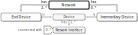
\includegraphics[scale=0.9]{figures/network}
  \caption{
    The meta model as a part of an ISO42010 architectural viewpoint.
  }
  \label{fig:iso42010}
\end{figure}